\documentclass[12pt] {article}
\usepackage{times}
\usepackage[margin=1in,bottom=1in,top=1in]{geometry}

\usepackage{hhline}

\usepackage{float}
\usepackage{graphicx}
\usepackage{subfig}
\usepackage{wrapfig,lipsum}
\usepackage{amssymb}
\usepackage{nath}
\usepackage{amsfonts}
\usepackage{hyperref}
\begin{document}

\title{TLP Project Report}
\author{Ahmed H. Mahmoud}
\date{}
\maketitle

%============table========
%\begin{figure}[tbh]
% \centering  
  
%\begin{tabular}{ |p{4cm}|| p{2cm}|p{2cm}|p{2cm}|p{2cm}|}
% \hline
% & Processor 1 &  Processor 2  & Processor 3 & Processor 4\\ \hhline{|=|=|=|=|=|}
% \hline
% Performance          &$1.08$        &$1.425$       &\textbf{1.52}  &   \\
% \hline
% Power (watts)        &$35.08$       &$34.88$       &\textbf{37.12} &   \\
% \hline 
% Area (units)         &$354$         &$352$         &$424$          &   \\
% \hline
% Cost (\$)            &\textbf{16.4} &$16.15$       &$28.23$        &   \\
% \hline
% Performance/area(\%) &$0.305$       &$0.404$       &$0.358$        &   \\
% \hline
% Performance/cost(\%) &$6.58$        &\textbf{8.82} &$5.38$         &   \\
% \hline
% CPI                  &\textbf{0.96} &  0.73        &$0.68$         &   \\
% \hline
%\end{tabular} 

%  \caption{Metric table for the four processors}
%   \label{tab:metric}
%\end{figure} 


%============Phtread========
\section{pthreads:}
The serial code was parallelized using pthreads by dividing the computation on number of threads. Since the 2D picture is mapped into 1D array (\emph{char* pic }), the 1D array elements were distributed to the number of threads specified by the user. Each thread carried the computation for certain number of elements and updated the globally-defined 1D array. The number of threads specified should be divisible by total number of elements. We tested varying number of threads and for each experiments we reported the performance (in msec) as shown in Figure \ref{fig:pth}. We can see that there is a range for which changing the number of threads does not affect the performance. This range is from $10-1920$ threads, given that that 2D picture is $1920\times 1920$. For higher than $1920$ threads, the cost of lunching more threads overcomes the actual computation. The best performance was obtained using $120$ threads which gave $415.097331$ mSec. 

\begin{figure}[!tbh]
 \centering        
   \subfloat [pthread]{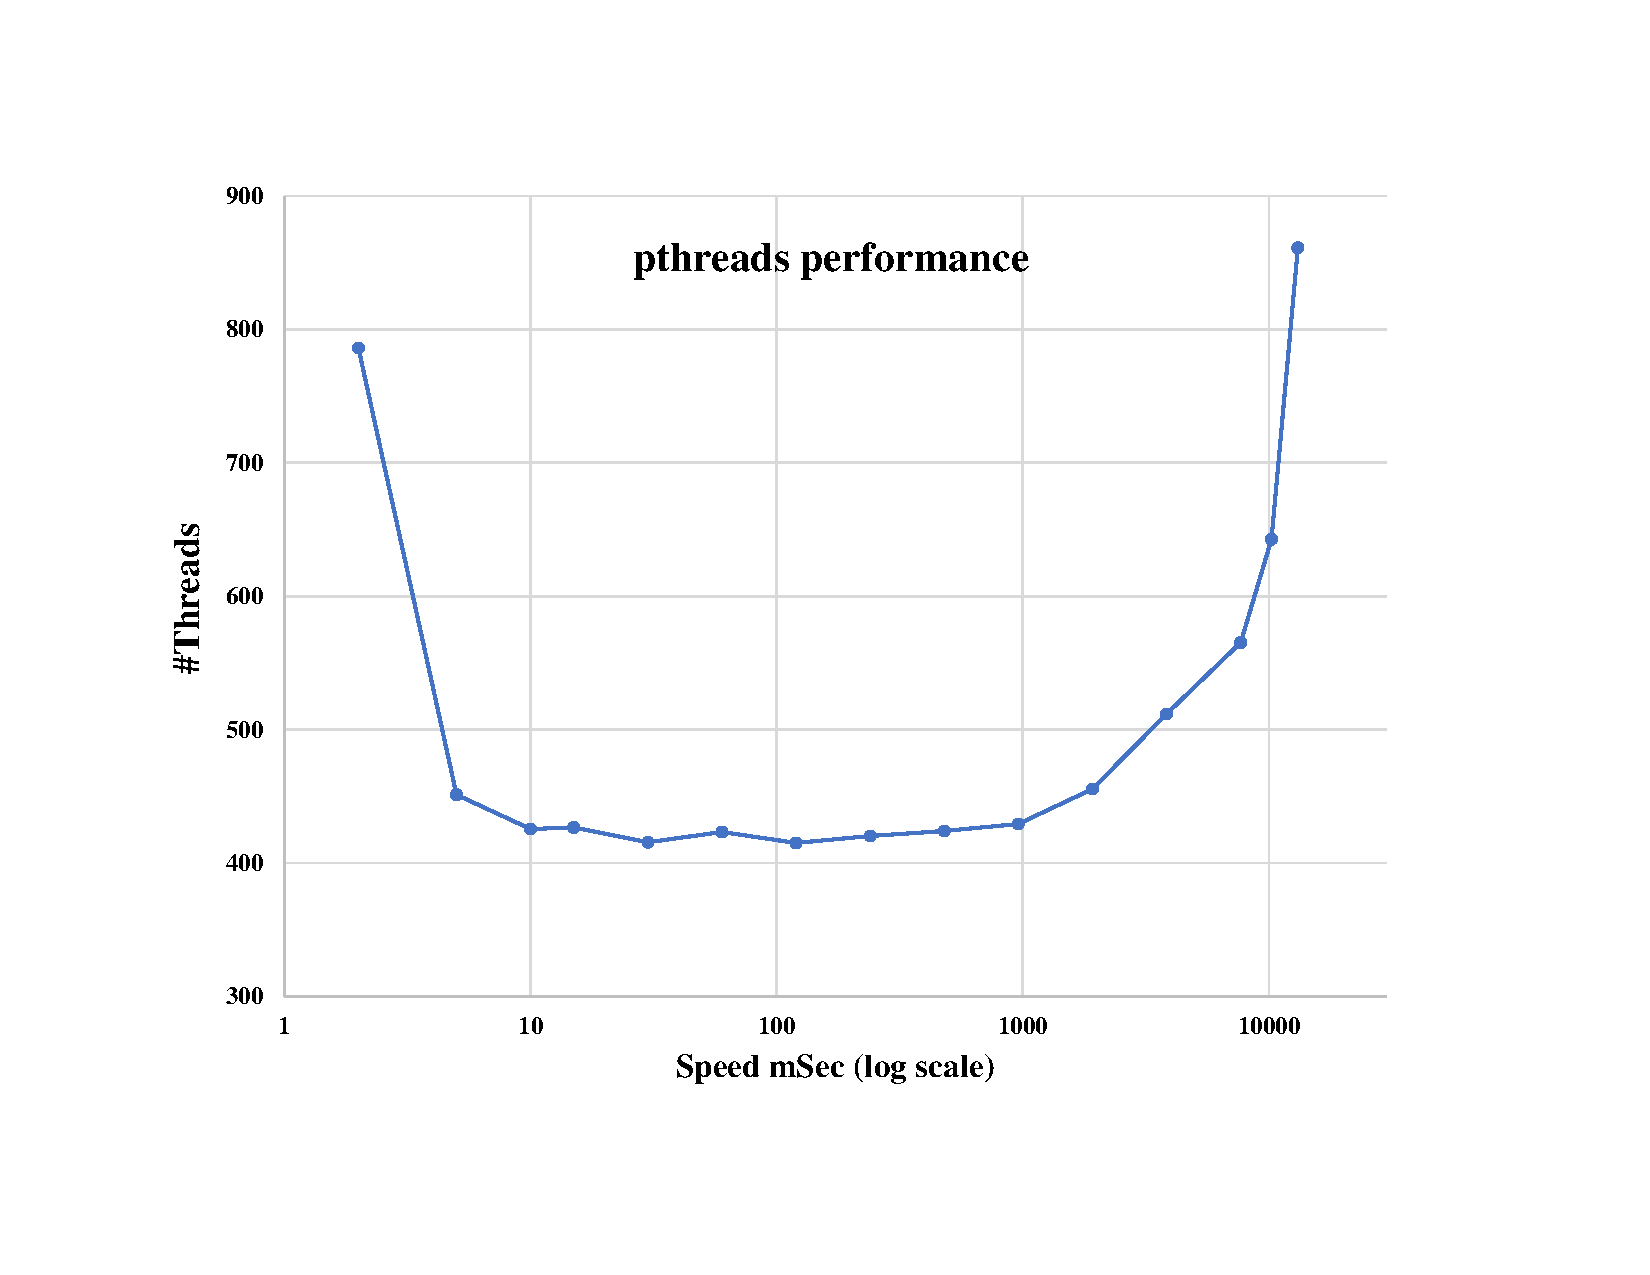
\includegraphics[width=0.5\textwidth]{pthreadfig.pdf}}
     \caption{Performance of pthreads using varying number of threads}
   \label{fig:pth}
\end{figure}  

%============MPI========
\section{MPI:}
The serial code was parallelized using MPI using master-slave approach. One processor was responsible of scattering the 1D array across the other processor and then gather the data after all processors have finished their assigned computation. Similar to the pthreads, each processor was responsible of updating a part in the 1D array as assigned by the master processor. We tested the performance for varying configuration as shown in Figure \ref{fig:mpi} where increasing the number of nodes is not always beneficial. The best performance can be obtained using 4 nodes where each node launch 4 processes with which the computation finishes in $427.4139$ mSec. This still does not outperform the speed up obtained from pthreads. 


\begin{figure}[!tbh]
 \centering        
   \subfloat [pthread]{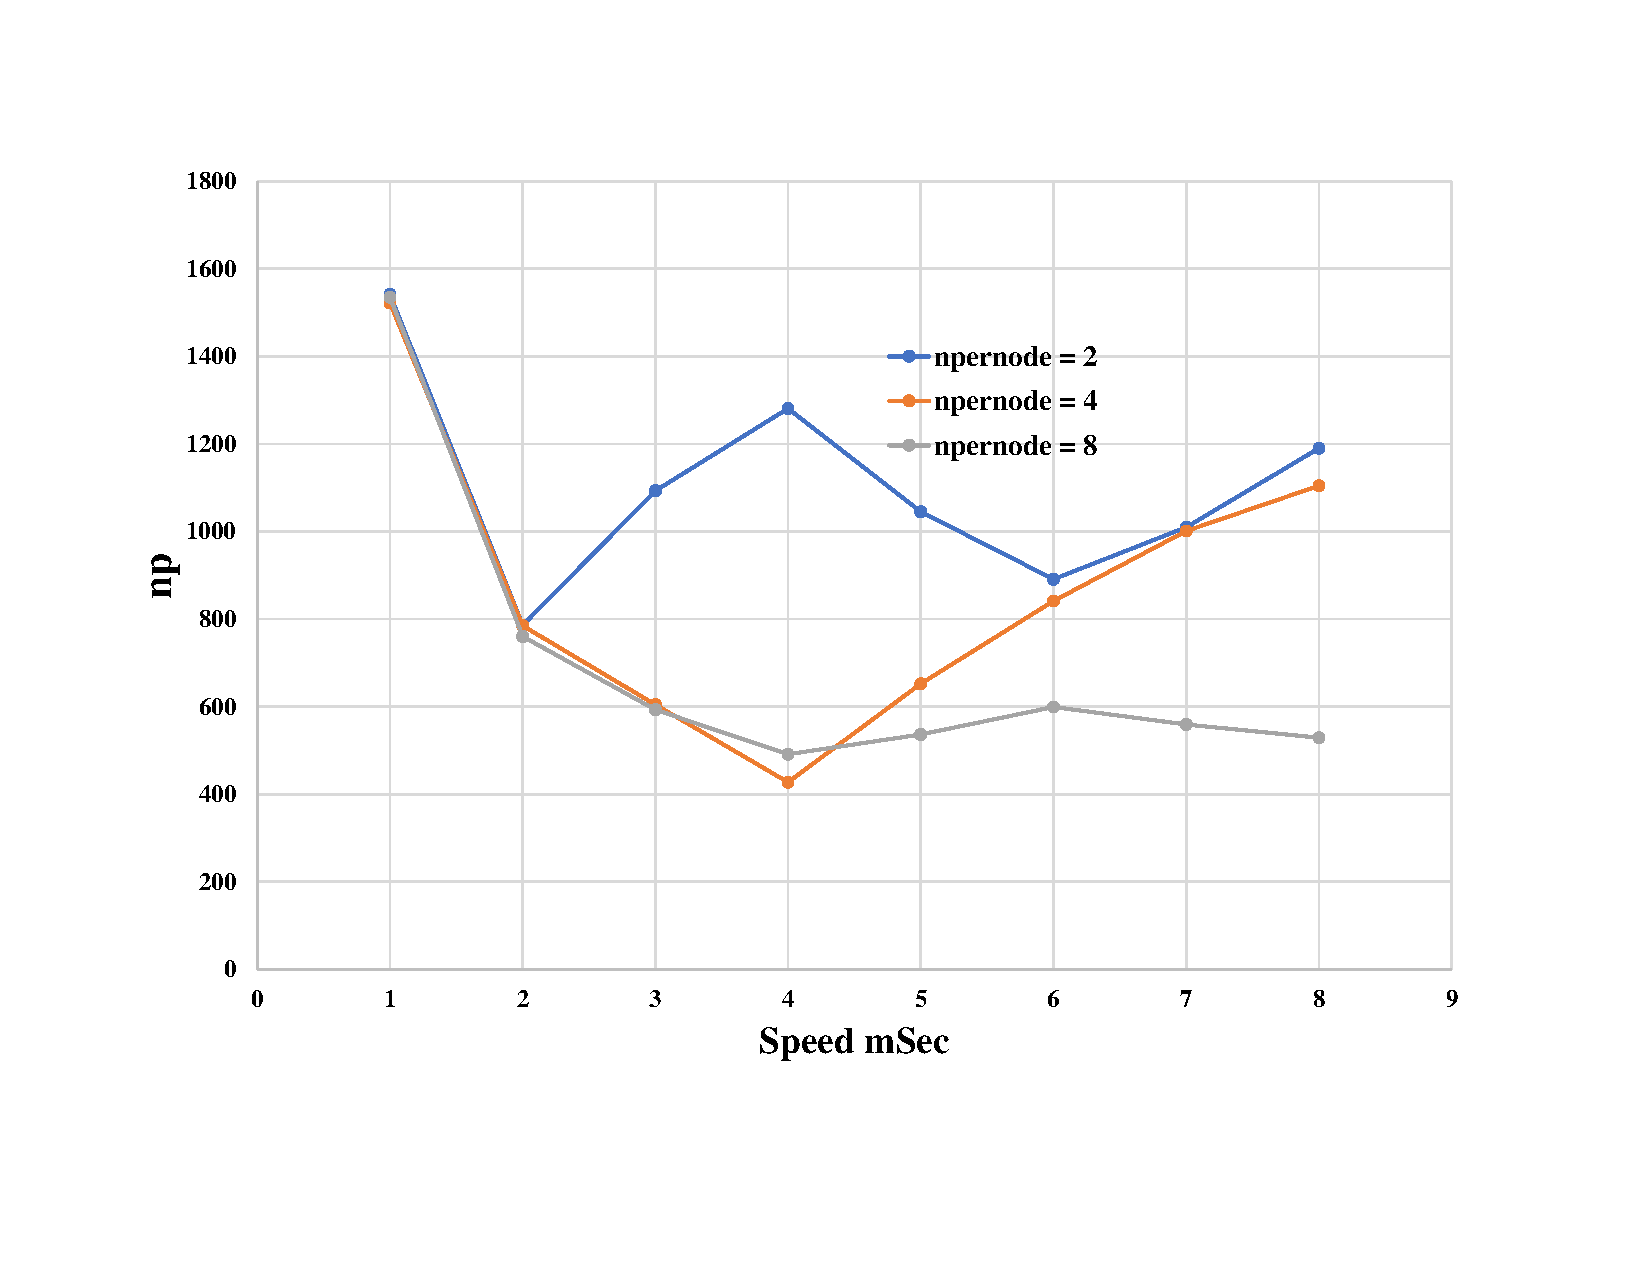
\includegraphics[width=0.5\textwidth]{mpifig.pdf}}
     \caption{Performance of MPI using varying processes per node (npernode) and number of processors (np)}
   \label{fig:mpi}
\end{figure} 


%============MPI vs Pthreads==========
\section{Comparison:}

By viewing the prices of dual-core Intel processors vs quad-core (https://en.wikipedia.org/

 wiki/List\_of\_Intel\_Core\_2\_microprocessors), we can see that the prices for the quad-core is almost $2.5$ times the dual-core one. Given the test program we run, since only a comparable performance can be obtained using 4 processors on MPI, we recommend to use dual-core thread-capable processor since it is more cost effective. 

\end{document}


 